\section{Introduction}

Cellular network reliability is increasingly managed through structured operational telemetry rather than isolated counters. A cell-level operations panel may contain continuous key performance indicator (KPI) and business counters, sparse alarm/fault events, anonymized cell identifiers, and time context. KPI histories describe load, accessibility, retainability, throughput and radio-quality dynamics; alarms mark discrete operational events; cell and time features encode persistent local behavior and periodic demand. Anticipatory mobile networking has shown that prediction can support proactive resource management \cite{bui2017anticipatory}. Deep-learning studies in mobile networks further connect traffic and performance prediction with data-driven control \cite{zhang2019deepmobile}. Recent O-RAN work stresses explainable, programmable radio access automation \cite{brik2025xaioran}, and mobile-traffic prediction studies show that cross-service correlations can carry useful forecasting information \cite{feng2024multiservice}. For cellular operations, proactive KPI degradation prediction is a reliability problem: the goal is to recognize deteriorating cell conditions before they become service-impacting events or costly manual troubleshooting cases.

The modeling difficulty lies in the heterogeneous form and uneven reliability of the available signals. KPI-history models can exploit strong temporal regularities, yet sparse event context is often part of the evidence that operators inspect during fault handling. Alarm/event models alone are also insufficient for continuous KPI prediction because alarms are rare and many KPI changes follow routine traffic or radio patterns rather than explicit faults. Prior cellular traffic work has emphasized spatial and temporal dependencies among base stations \cite{wang2017spatiotemporal}, while recent mobile traffic forecasting studies show the importance of network-wide temporal patterns \cite{sun2022mobiletraffic}. Classic alarm-correlation work has long noted that a single fault may generate many related alarms \cite{jakobson1993alarm}; communication-network fault-identification studies also show that alarm floods complicate localization \cite{bouloutas1994alarm}. Enterprise operations data add further constraints: physical topology may be unavailable, expert root-cause annotations may be absent, and data release may be restricted by business and network-operation confidentiality.

This paper studies alarm-aware KPI degradation prediction using an anonymized real-world mobile broadband (MBB) operations dataset provided by Huawei Technologies. The source collection covers approximately 500 cellular sites, while the aligned panel evaluated in this study contains 33 anonymized cell entities without geographically identifiable site information. We propose CET-STGL as a causal-inspired event-token spatio-temporal framework for this setting. The central methodological idea is a temporally admissible representation of heterogeneous cellular telemetry: KPI histories are transformed into local patch features, alarms are represented through sparse event and intensity features, and alarm-degradation associations are incorporated as train-only event influence priors. When physical topology is unavailable, cross-cell context is inferred from training-period operational correlations. CET-STGL organizes operational signals under realistic monitoring constraints, without treating observed associations as causal evidence or expert-verified fault localization.
The reliability-oriented pipeline and the main guardrails used throughout the paper are summarized in Fig.~\ref{fig:cet_stgl_overview}.

\begin{figure}[!t]
    \centering
    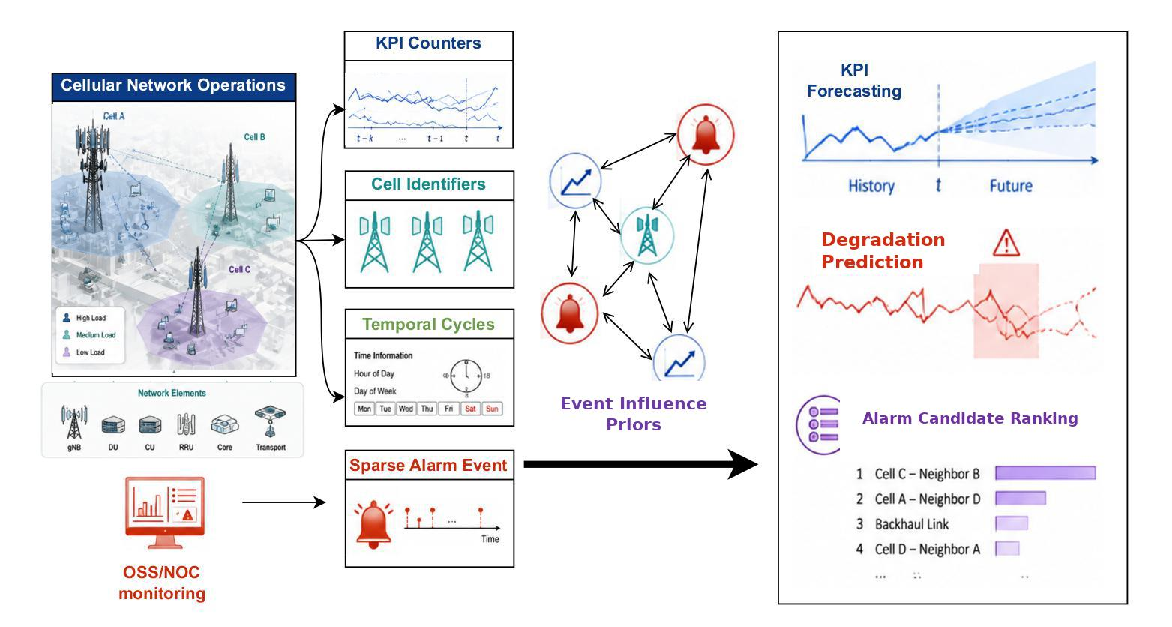
\includegraphics[width=0.98\textwidth]{figures/Fig0_cet_stgl_reliability_overview.pdf}
    \caption{Overview of CET-STGL from reliability-oriented cellular network operations to analysis.}
    \label{fig:cet_stgl_overview}
\end{figure}

Recent telecom LLM discussions examine language models for telecommunications \cite{maatouk2025llmtelecom}. Domain-adapted telecom LLMs focus on language and standards knowledge \cite{zou2025telecomgpt}, and networking LLM systems study adaptation to networking tasks \cite{wu2024netllm}. Benchmark proposals for industrial telecom workflows provide a separate line of context \cite{xiao2026telecombench}. This paper instead works with structured telemetry for cellular reliability analysis, with KPI forecasting, weak degradation classification and weak alarm-candidate prioritization evaluated on a private operations slice. Section~\ref{sec:limitations_reproducibility} states the limits on causality, expert RCA validation and end-to-end neural spatio-temporal graph evaluation.

The paper makes four contributions:
\begin{enumerate}
    \item Alarm-aware KPI degradation prediction is formulated as a multi-task evaluation problem over real cellular KPI/business and alarm/fault panels.
    \item A temporally admissible, causal-inspired event-token representation is formalised that aligns KPI patch features, alarm event features, cell/time context, train-only event influence priors and inferred cross-cell context.
    \item A leakage-controlled reliability evaluation protocol is provided for 1/3/6/12-hour KPI forecasting, weak degradation classification and weak alarm-candidate prioritization.
    \item The empirical findings are narrow by design: KPI-history baselines remain strong, event-intensity variants are weak standalone predictors, the evaluated lightweight CET-STGL instantiation is competitive on several primary-KPI forecasting metrics, and gains from alarm and graph features are limited and non-uniform under the current weak-label protocol.
\end{enumerate}

The remainder of this paper is organized as follows. Section~\ref{sec:related_work} reviews related work. Section~\ref{sec:problem_method} formulates the tasks. Section~\ref{sec:methodology} presents CET-STGL. Section~\ref{sec:experimental_evaluation} reports the experimental evaluation and limitations. Section~\ref{sec:conclusion} concludes the paper.
